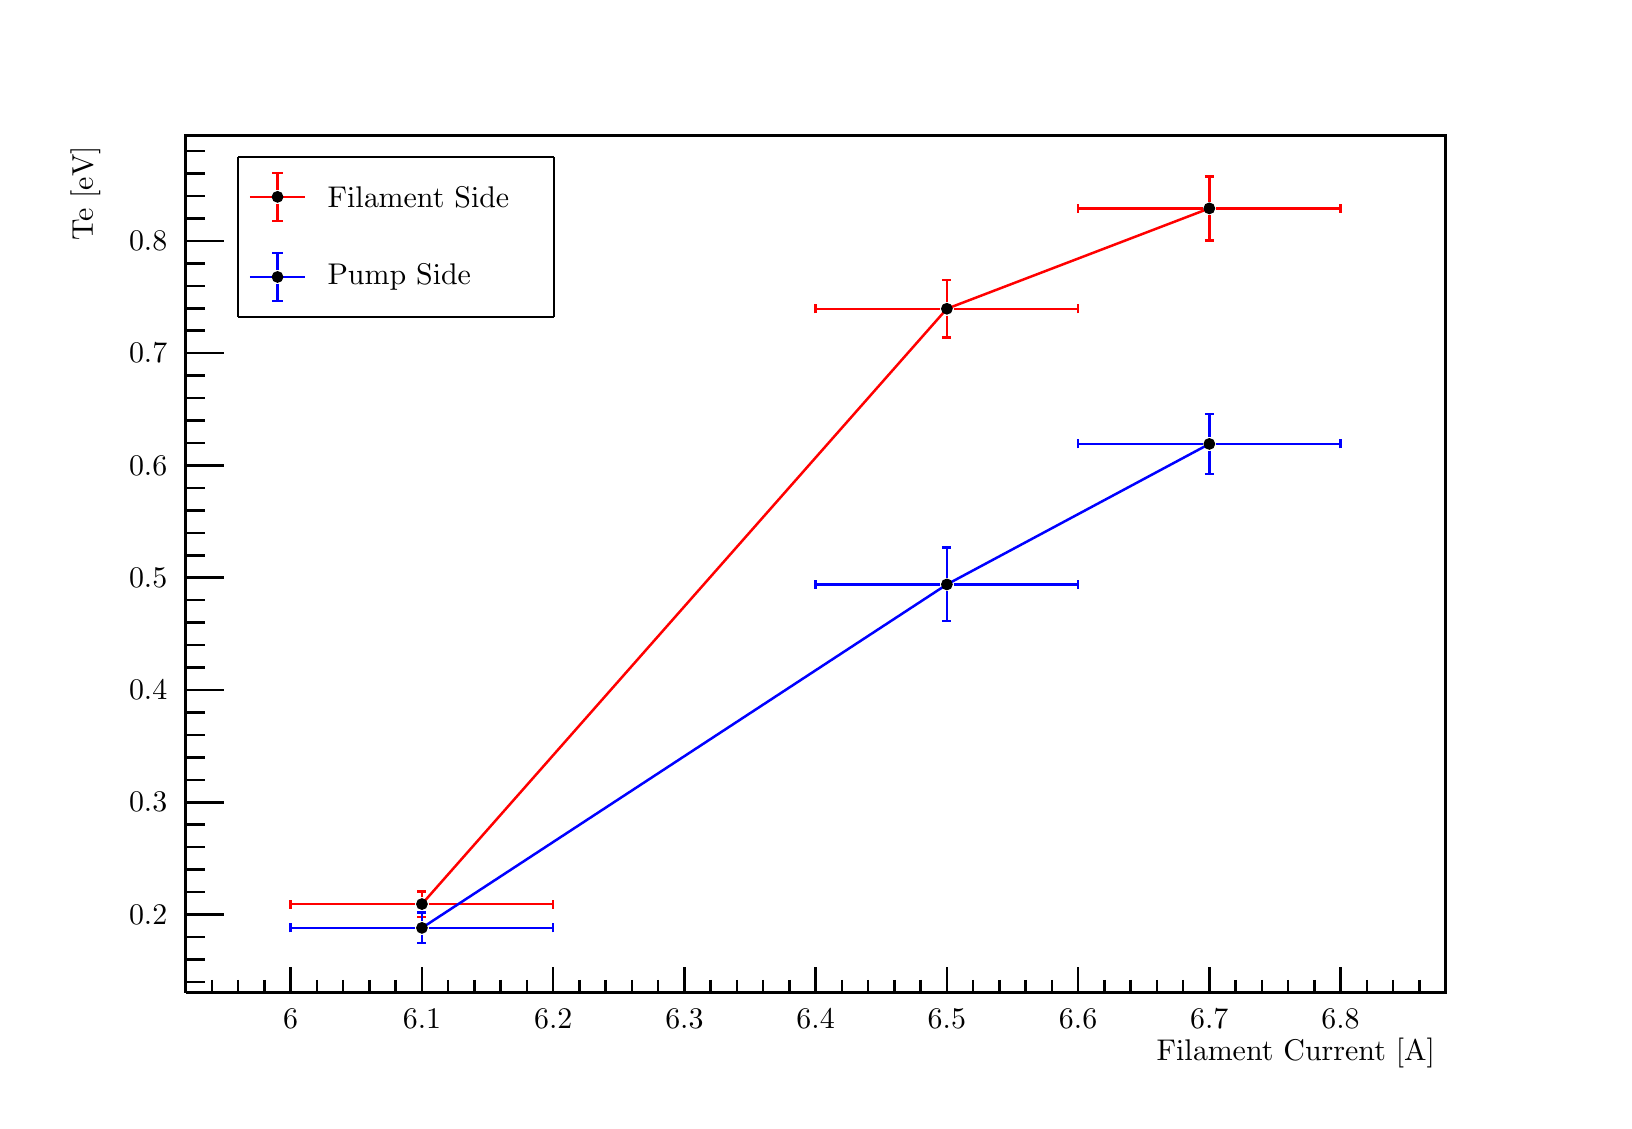
\begin{tikzpicture}
\pgfdeclareplotmark{cross} {
\pgfpathmoveto{\pgfpoint{-0.3\pgfplotmarksize}{\pgfplotmarksize}}
\pgfpathlineto{\pgfpoint{+0.3\pgfplotmarksize}{\pgfplotmarksize}}
\pgfpathlineto{\pgfpoint{+0.3\pgfplotmarksize}{0.3\pgfplotmarksize}}
\pgfpathlineto{\pgfpoint{+1\pgfplotmarksize}{0.3\pgfplotmarksize}}
\pgfpathlineto{\pgfpoint{+1\pgfplotmarksize}{-0.3\pgfplotmarksize}}
\pgfpathlineto{\pgfpoint{+0.3\pgfplotmarksize}{-0.3\pgfplotmarksize}}
\pgfpathlineto{\pgfpoint{+0.3\pgfplotmarksize}{-1.\pgfplotmarksize}}
\pgfpathlineto{\pgfpoint{-0.3\pgfplotmarksize}{-1.\pgfplotmarksize}}
\pgfpathlineto{\pgfpoint{-0.3\pgfplotmarksize}{-0.3\pgfplotmarksize}}
\pgfpathlineto{\pgfpoint{-1.\pgfplotmarksize}{-0.3\pgfplotmarksize}}
\pgfpathlineto{\pgfpoint{-1.\pgfplotmarksize}{0.3\pgfplotmarksize}}
\pgfpathlineto{\pgfpoint{-0.3\pgfplotmarksize}{0.3\pgfplotmarksize}}
\pgfpathclose
\pgfusepathqstroke
}
\pgfdeclareplotmark{cross*} {
\pgfpathmoveto{\pgfpoint{-0.3\pgfplotmarksize}{\pgfplotmarksize}}
\pgfpathlineto{\pgfpoint{+0.3\pgfplotmarksize}{\pgfplotmarksize}}
\pgfpathlineto{\pgfpoint{+0.3\pgfplotmarksize}{0.3\pgfplotmarksize}}
\pgfpathlineto{\pgfpoint{+1\pgfplotmarksize}{0.3\pgfplotmarksize}}
\pgfpathlineto{\pgfpoint{+1\pgfplotmarksize}{-0.3\pgfplotmarksize}}
\pgfpathlineto{\pgfpoint{+0.3\pgfplotmarksize}{-0.3\pgfplotmarksize}}
\pgfpathlineto{\pgfpoint{+0.3\pgfplotmarksize}{-1.\pgfplotmarksize}}
\pgfpathlineto{\pgfpoint{-0.3\pgfplotmarksize}{-1.\pgfplotmarksize}}
\pgfpathlineto{\pgfpoint{-0.3\pgfplotmarksize}{-0.3\pgfplotmarksize}}
\pgfpathlineto{\pgfpoint{-1.\pgfplotmarksize}{-0.3\pgfplotmarksize}}
\pgfpathlineto{\pgfpoint{-1.\pgfplotmarksize}{0.3\pgfplotmarksize}}
\pgfpathlineto{\pgfpoint{-0.3\pgfplotmarksize}{0.3\pgfplotmarksize}}
\pgfpathclose
\pgfusepathqfillstroke
}
\pgfdeclareplotmark{newstar} {
\pgfpathmoveto{\pgfqpoint{0pt}{\pgfplotmarksize}}
\pgfpathlineto{\pgfqpointpolar{44}{0.5\pgfplotmarksize}}
\pgfpathlineto{\pgfqpointpolar{18}{\pgfplotmarksize}}
\pgfpathlineto{\pgfqpointpolar{-20}{0.5\pgfplotmarksize}}
\pgfpathlineto{\pgfqpointpolar{-54}{\pgfplotmarksize}}
\pgfpathlineto{\pgfqpointpolar{-90}{0.5\pgfplotmarksize}}
\pgfpathlineto{\pgfqpointpolar{234}{\pgfplotmarksize}}
\pgfpathlineto{\pgfqpointpolar{198}{0.5\pgfplotmarksize}}
\pgfpathlineto{\pgfqpointpolar{162}{\pgfplotmarksize}}
\pgfpathlineto{\pgfqpointpolar{134}{0.5\pgfplotmarksize}}
\pgfpathclose
\pgfusepathqstroke
}
\pgfdeclareplotmark{newstar*} {
\pgfpathmoveto{\pgfqpoint{0pt}{\pgfplotmarksize}}
\pgfpathlineto{\pgfqpointpolar{44}{0.5\pgfplotmarksize}}
\pgfpathlineto{\pgfqpointpolar{18}{\pgfplotmarksize}}
\pgfpathlineto{\pgfqpointpolar{-20}{0.5\pgfplotmarksize}}
\pgfpathlineto{\pgfqpointpolar{-54}{\pgfplotmarksize}}
\pgfpathlineto{\pgfqpointpolar{-90}{0.5\pgfplotmarksize}}
\pgfpathlineto{\pgfqpointpolar{234}{\pgfplotmarksize}}
\pgfpathlineto{\pgfqpointpolar{198}{0.5\pgfplotmarksize}}
\pgfpathlineto{\pgfqpointpolar{162}{\pgfplotmarksize}}
\pgfpathlineto{\pgfqpointpolar{134}{0.5\pgfplotmarksize}}
\pgfpathclose
\pgfusepathqfillstroke
}
\definecolor{c}{rgb}{1,1,1};
\draw [color=c, fill=c] (0,0) rectangle (20,13.6103);
\draw [color=c, fill=c] (2,1.36103) rectangle (18,12.2493);
\definecolor{c}{rgb}{0,0,0};
\draw [c,line width=0.9] (2,1.36103) -- (2,12.2493) -- (18,12.2493) -- (18,1.36103) -- (2,1.36103);
\definecolor{c}{rgb}{1,1,1};
\draw [color=c, fill=c] (2,1.36103) rectangle (18,12.2493);
\definecolor{c}{rgb}{0,0,0};
\draw [c,line width=0.9] (2,1.36103) -- (2,12.2493) -- (18,12.2493) -- (18,1.36103) -- (2,1.36103);
\draw [c,line width=0.9] (2,1.36103) -- (18,1.36103);
\draw [c,line width=0.9] (3.33333,1.68768) -- (3.33333,1.36103);
\draw [c,line width=0.9] (3.66667,1.52436) -- (3.66667,1.36103);
\draw [c,line width=0.9] (4,1.52436) -- (4,1.36103);
\draw [c,line width=0.9] (4.33333,1.52436) -- (4.33333,1.36103);
\draw [c,line width=0.9] (4.66667,1.52436) -- (4.66667,1.36103);
\draw [c,line width=0.9] (5,1.68768) -- (5,1.36103);
\draw [c,line width=0.9] (5.33333,1.52436) -- (5.33333,1.36103);
\draw [c,line width=0.9] (5.66667,1.52436) -- (5.66667,1.36103);
\draw [c,line width=0.9] (6,1.52436) -- (6,1.36103);
\draw [c,line width=0.9] (6.33333,1.52436) -- (6.33333,1.36103);
\draw [c,line width=0.9] (6.66667,1.68768) -- (6.66667,1.36103);
\draw [c,line width=0.9] (7,1.52436) -- (7,1.36103);
\draw [c,line width=0.9] (7.33333,1.52436) -- (7.33333,1.36103);
\draw [c,line width=0.9] (7.66667,1.52436) -- (7.66667,1.36103);
\draw [c,line width=0.9] (8,1.52436) -- (8,1.36103);
\draw [c,line width=0.9] (8.33333,1.68768) -- (8.33333,1.36103);
\draw [c,line width=0.9] (8.66667,1.52436) -- (8.66667,1.36103);
\draw [c,line width=0.9] (9,1.52436) -- (9,1.36103);
\draw [c,line width=0.9] (9.33333,1.52436) -- (9.33333,1.36103);
\draw [c,line width=0.9] (9.66667,1.52436) -- (9.66667,1.36103);
\draw [c,line width=0.9] (10,1.68768) -- (10,1.36103);
\draw [c,line width=0.9] (10.3333,1.52436) -- (10.3333,1.36103);
\draw [c,line width=0.9] (10.6667,1.52436) -- (10.6667,1.36103);
\draw [c,line width=0.9] (11,1.52436) -- (11,1.36103);
\draw [c,line width=0.9] (11.3333,1.52436) -- (11.3333,1.36103);
\draw [c,line width=0.9] (11.6667,1.68768) -- (11.6667,1.36103);
\draw [c,line width=0.9] (12,1.52436) -- (12,1.36103);
\draw [c,line width=0.9] (12.3333,1.52436) -- (12.3333,1.36103);
\draw [c,line width=0.9] (12.6667,1.52436) -- (12.6667,1.36103);
\draw [c,line width=0.9] (13,1.52436) -- (13,1.36103);
\draw [c,line width=0.9] (13.3333,1.68768) -- (13.3333,1.36103);
\draw [c,line width=0.9] (13.6667,1.52436) -- (13.6667,1.36103);
\draw [c,line width=0.9] (14,1.52436) -- (14,1.36103);
\draw [c,line width=0.9] (14.3333,1.52436) -- (14.3333,1.36103);
\draw [c,line width=0.9] (14.6667,1.52436) -- (14.6667,1.36103);
\draw [c,line width=0.9] (15,1.68768) -- (15,1.36103);
\draw [c,line width=0.9] (15.3333,1.52436) -- (15.3333,1.36103);
\draw [c,line width=0.9] (15.6667,1.52436) -- (15.6667,1.36103);
\draw [c,line width=0.9] (16,1.52436) -- (16,1.36103);
\draw [c,line width=0.9] (16.3333,1.52436) -- (16.3333,1.36103);
\draw [c,line width=0.9] (16.6667,1.68768) -- (16.6667,1.36103);
\draw [c,line width=0.9] (3.33333,1.68768) -- (3.33333,1.36103);
\draw [c,line width=0.9] (3,1.52436) -- (3,1.36103);
\draw [c,line width=0.9] (2.66667,1.52436) -- (2.66667,1.36103);
\draw [c,line width=0.9] (2.33333,1.52436) -- (2.33333,1.36103);
\draw [c,line width=0.9] (2,1.52436) -- (2,1.36103);
\draw [c,line width=0.9] (16.6667,1.68768) -- (16.6667,1.36103);
\draw [c,line width=0.9] (17,1.52436) -- (17,1.36103);
\draw [c,line width=0.9] (17.3333,1.52436) -- (17.3333,1.36103);
\draw [c,line width=0.9] (17.6667,1.52436) -- (17.6667,1.36103);
\draw [anchor=base] (3.33333,0.911891) node[scale=1.08185, color=c, rotate=0]{6};
\draw [anchor=base] (5,0.911891) node[scale=1.08185, color=c, rotate=0]{6.1};
\draw [anchor=base] (6.66667,0.911891) node[scale=1.08185, color=c, rotate=0]{6.2};
\draw [anchor=base] (8.33333,0.911891) node[scale=1.08185, color=c, rotate=0]{6.3};
\draw [anchor=base] (10,0.911891) node[scale=1.08185, color=c, rotate=0]{6.4};
\draw [anchor=base] (11.6667,0.911891) node[scale=1.08185, color=c, rotate=0]{6.5};
\draw [anchor=base] (13.3333,0.911891) node[scale=1.08185, color=c, rotate=0]{6.6};
\draw [anchor=base] (15,0.911891) node[scale=1.08185, color=c, rotate=0]{6.7};
\draw [anchor=base] (16.6667,0.911891) node[scale=1.08185, color=c, rotate=0]{6.8};
\draw [anchor= east] (18,0.598854) node[scale=1.08185, color=c, rotate=0]{Filament Current [A]};
\draw [c,line width=0.9] (2,1.36103) -- (2,12.2493);
\draw [c,line width=0.9] (2.48,2.35424) -- (2,2.35424);
\draw [c,line width=0.9] (2.24,2.6394) -- (2,2.6394);
\draw [c,line width=0.9] (2.24,2.92457) -- (2,2.92457);
\draw [c,line width=0.9] (2.24,3.20973) -- (2,3.20973);
\draw [c,line width=0.9] (2.24,3.49489) -- (2,3.49489);
\draw [c,line width=0.9] (2.48,3.78006) -- (2,3.78006);
\draw [c,line width=0.9] (2.24,4.06522) -- (2,4.06522);
\draw [c,line width=0.9] (2.24,4.35038) -- (2,4.35038);
\draw [c,line width=0.9] (2.24,4.63555) -- (2,4.63555);
\draw [c,line width=0.9] (2.24,4.92071) -- (2,4.92071);
\draw [c,line width=0.9] (2.48,5.20587) -- (2,5.20587);
\draw [c,line width=0.9] (2.24,5.49103) -- (2,5.49103);
\draw [c,line width=0.9] (2.24,5.7762) -- (2,5.7762);
\draw [c,line width=0.9] (2.24,6.06136) -- (2,6.06136);
\draw [c,line width=0.9] (2.24,6.34652) -- (2,6.34652);
\draw [c,line width=0.9] (2.48,6.63169) -- (2,6.63169);
\draw [c,line width=0.9] (2.24,6.91685) -- (2,6.91685);
\draw [c,line width=0.9] (2.24,7.20201) -- (2,7.20201);
\draw [c,line width=0.9] (2.24,7.48718) -- (2,7.48718);
\draw [c,line width=0.9] (2.24,7.77234) -- (2,7.77234);
\draw [c,line width=0.9] (2.48,8.0575) -- (2,8.0575);
\draw [c,line width=0.9] (2.24,8.34266) -- (2,8.34266);
\draw [c,line width=0.9] (2.24,8.62783) -- (2,8.62783);
\draw [c,line width=0.9] (2.24,8.91299) -- (2,8.91299);
\draw [c,line width=0.9] (2.24,9.19815) -- (2,9.19815);
\draw [c,line width=0.9] (2.48,9.48332) -- (2,9.48332);
\draw [c,line width=0.9] (2.24,9.76848) -- (2,9.76848);
\draw [c,line width=0.9] (2.24,10.0536) -- (2,10.0536);
\draw [c,line width=0.9] (2.24,10.3388) -- (2,10.3388);
\draw [c,line width=0.9] (2.24,10.624) -- (2,10.624);
\draw [c,line width=0.9] (2.48,10.9091) -- (2,10.9091);
\draw [c,line width=0.9] (2.48,2.35424) -- (2,2.35424);
\draw [c,line width=0.9] (2.24,2.06908) -- (2,2.06908);
\draw [c,line width=0.9] (2.24,1.78391) -- (2,1.78391);
\draw [c,line width=0.9] (2.24,1.49875) -- (2,1.49875);
\draw [c,line width=0.9] (2.48,10.9091) -- (2,10.9091);
\draw [c,line width=0.9] (2.24,11.1943) -- (2,11.1943);
\draw [c,line width=0.9] (2.24,11.4795) -- (2,11.4795);
\draw [c,line width=0.9] (2.24,11.7646) -- (2,11.7646);
\draw [c,line width=0.9] (2.24,12.0498) -- (2,12.0498);
\draw [anchor= east] (1.9,2.35424) node[scale=1.08185, color=c, rotate=0]{0.2};
\draw [anchor= east] (1.9,3.78006) node[scale=1.08185, color=c, rotate=0]{0.3};
\draw [anchor= east] (1.9,5.20587) node[scale=1.08185, color=c, rotate=0]{0.4};
\draw [anchor= east] (1.9,6.63169) node[scale=1.08185, color=c, rotate=0]{0.5};
\draw [anchor= east] (1.9,8.0575) node[scale=1.08185, color=c, rotate=0]{0.6};
\draw [anchor= east] (1.9,9.48332) node[scale=1.08185, color=c, rotate=0]{0.7};
\draw [anchor= east] (1.9,10.9091) node[scale=1.08185, color=c, rotate=0]{0.8};
\draw [anchor= east] (0.726934,12.2493) node[scale=1.08185, color=c, rotate=90]{Te [eV]};
\definecolor{c}{rgb}{1,0,0};
\draw [c,line width=0.9] (5,2.4871) -- (11.6667,10.0475) -- (15,11.3222);
\definecolor{c}{rgb}{0,0,0};
\foreach \P in {(5,2.4871), (11.6667,10.0475), (15,11.3222)}{\draw[mark options={color=c,fill=c},mark size=1.921922pt,mark=*] plot coordinates {\P};}
\definecolor{c}{rgb}{1,0,0};
\draw [c,line width=0.9] (4.91404,2.4871) -- (3.33333,2.4871);
\draw [c,line width=0.9] (3.33333,2.42979) -- (3.33333,2.5444);
\draw [c,line width=0.9] (5.08596,2.4871) -- (6.66667,2.4871);
\draw [c,line width=0.9] (6.66667,2.42979) -- (6.66667,2.5444);
\draw [c,line width=0.9] (5,2.57306) -- (5,2.6495);
\draw [c,line width=0.9] (4.94269,2.6495) -- (5.05731,2.6495);
\draw [c,line width=0.9] (5,2.40114) -- (5,2.3247);
\draw [c,line width=0.9] (4.94269,2.3247) -- (5.05731,2.3247);
\draw [c,line width=0.9] (11.5807,10.0475) -- (10,10.0475);
\draw [c,line width=0.9] (10,9.99023) -- (10,10.1048);
\draw [c,line width=0.9] (11.7526,10.0475) -- (13.3333,10.0475);
\draw [c,line width=0.9] (13.3333,9.99023) -- (13.3333,10.1048);
\draw [c,line width=0.9] (11.6667,10.1335) -- (11.6667,10.4143);
\draw [c,line width=0.9] (11.6094,10.4143) -- (11.724,10.4143);
\draw [c,line width=0.9] (11.6667,9.96158) -- (11.6667,9.68076);
\draw [c,line width=0.9] (11.6094,9.68076) -- (11.724,9.68076);
\draw [c,line width=0.9] (14.914,11.3222) -- (13.3333,11.3222);
\draw [c,line width=0.9] (13.3333,11.2649) -- (13.3333,11.3795);
\draw [c,line width=0.9] (15.086,11.3222) -- (16.6667,11.3222);
\draw [c,line width=0.9] (16.6667,11.2649) -- (16.6667,11.3795);
\draw [c,line width=0.9] (15,11.4081) -- (15,11.729);
\draw [c,line width=0.9] (14.9427,11.729) -- (15.0573,11.729);
\draw [c,line width=0.9] (15,11.2362) -- (15,10.9153);
\draw [c,line width=0.9] (14.9427,10.9153) -- (15.0573,10.9153);
\definecolor{c}{rgb}{0,0,1};
\draw [c,line width=0.9] (4.91404,2.18463) -- (3.33333,2.18463);
\draw [c,line width=0.9] (3.33333,2.12732) -- (3.33333,2.24193);
\draw [c,line width=0.9] (5.08596,2.18463) -- (6.66667,2.18463);
\draw [c,line width=0.9] (6.66667,2.12732) -- (6.66667,2.24193);
\draw [c,line width=0.9] (5,2.27059) -- (5,2.37785);
\draw [c,line width=0.9] (4.94269,2.37785) -- (5.05731,2.37785);
\draw [c,line width=0.9] (5,2.09867) -- (5,1.9914);
\draw [c,line width=0.9] (4.94269,1.9914) -- (5.05731,1.9914);
\draw [c,line width=0.9] (11.5807,6.54642) -- (10,6.54642);
\draw [c,line width=0.9] (10,6.48912) -- (10,6.60373);
\draw [c,line width=0.9] (11.7526,6.54642) -- (13.3333,6.54642);
\draw [c,line width=0.9] (13.3333,6.48912) -- (13.3333,6.60373);
\draw [c,line width=0.9] (11.6667,6.63238) -- (11.6667,7.01387);
\draw [c,line width=0.9] (11.6094,7.01387) -- (11.724,7.01387);
\draw [c,line width=0.9] (11.6667,6.46046) -- (11.6667,6.07897);
\draw [c,line width=0.9] (11.6094,6.07897) -- (11.724,6.07897);
\draw [c,line width=0.9] (14.914,8.33079) -- (13.3333,8.33079);
\draw [c,line width=0.9] (13.3333,8.27348) -- (13.3333,8.38809);
\draw [c,line width=0.9] (15.086,8.33079) -- (16.6667,8.33079);
\draw [c,line width=0.9] (16.6667,8.27348) -- (16.6667,8.38809);
\draw [c,line width=0.9] (15,8.41675) -- (15,8.71281);
\draw [c,line width=0.9] (14.9427,8.71281) -- (15.0573,8.71281);
\draw [c,line width=0.9] (15,8.24483) -- (15,7.94876);
\draw [c,line width=0.9] (14.9427,7.94876) -- (15.0573,7.94876);
\draw [c,line width=0.9] (5,2.18463) -- (11.6667,6.54642) -- (15,8.33079);
\definecolor{c}{rgb}{0,0,0};
\foreach \P in {(5,2.18463), (11.6667,6.54642), (15,8.33079)}{\draw[mark options={color=c,fill=c},mark size=1.921922pt,mark=*] plot coordinates {\P};}
\definecolor{c}{rgb}{1,1,1};
\draw [color=c, fill=c] (2.66476,9.94269) rectangle (6.67622,11.9771);
\definecolor{c}{rgb}{0,0,0};
\draw [c,line width=0.9] (2.66476,9.94269) -- (6.67622,9.94269);
\draw [c,line width=0.9] (6.67622,9.94269) -- (6.67622,11.9771);
\draw [c,line width=0.9] (6.67622,11.9771) -- (2.66476,11.9771);
\draw [c,line width=0.9] (2.66476,11.9771) -- (2.66476,9.94269);
\draw [anchor= west] (3.66762,11.4685) node[scale=1.08185, color=c, rotate=0]{Filament Side};
\definecolor{c}{rgb}{1,0,0};
\draw [c,line width=0.9] (2.81519,11.4685) -- (3.51719,11.4685);
\draw [c,line width=0.9] (3.16619,11.5544) -- (3.16619,11.7736);
\draw [c,line width=0.9] (3.16619,11.3825) -- (3.16619,11.1633);
\draw [c,line width=0.9] (3.09599,11.7736) -- (3.23639,11.7736);
\draw [c,line width=0.9] (3.09599,11.1633) -- (3.23639,11.1633);
\definecolor{c}{rgb}{0,0,0};
\foreach \P in {(3.16619,11.4685)}{\draw[mark options={color=c,fill=c},mark size=1.921922pt,mark=*] plot coordinates {\P};}
\draw [anchor= west] (3.66762,10.4513) node[scale=1.08185, color=c, rotate=0]{Pump Side};
\definecolor{c}{rgb}{0,0,1};
\draw [c,line width=0.9] (2.81519,10.4513) -- (3.51719,10.4513);
\draw [c,line width=0.9] (3.16619,10.5372) -- (3.16619,10.7564);
\draw [c,line width=0.9] (3.16619,10.3653) -- (3.16619,10.1461);
\draw [c,line width=0.9] (3.09599,10.7564) -- (3.23639,10.7564);
\draw [c,line width=0.9] (3.09599,10.1461) -- (3.23639,10.1461);
\definecolor{c}{rgb}{0,0,0};
\foreach \P in {(3.16619,10.4513)}{\draw[mark options={color=c,fill=c},mark size=1.921922pt,mark=*] plot coordinates {\P};}
\end{tikzpicture}
